\section{Vertrauliche Kommunikation}
\label{subsec:vertrauliche_kommunikation}


Die Kommunikation zwischen den Teilnehmern soll vertraulich sein. Das bedeutet, dass die Nachrichten nur von den Teilnehmern gelesen werden können, die an der Kommunikation beteiligt sind. Um dies gewährleisten zu können, wird eine Ende-zu-Ende-Verschlüsselung verwendet. Das in Abschnitt \ref{subsec:signal_protokoll_basics} \textit{\nameref{subsec:signal_protokoll_basics}} besprochene Signal-Protokoll ist momentan der Industriestandard für Ende-zu-Ende-Verschlüs-\\selung und wird von den bekanntesten Messengern verwendet \Parencite[S. 260]{Wong_KryptoPraxis}. 

Deshalb soll dieses Protokoll auch für die Sicherheit der Kommunikation in dieser Arbeit verwendet werden. Allerdings ist das Signal-Protokoll auf eine Client-Server-Architektur ausgelegt. Da in dieser Arbeit eine Peer-to-Peer-Architektur verwendet wird, muss das Signal-Protokoll angepasst werden.

Der Double Ratchet Algorithmus (siehe \ref{subsec:signal_protokoll_basics} \textit{\nameref{subsec:signal_protokoll_basics}}) wird übernommen. Damit wird die \textit{Forward Secrecy} gewährleistet. Der X3DH-Schlüsselaus-\\tausch kann allerdings nicht verwendet werden.  

\subsection{Schlüsselvereinbarung}
Für die Implementierung eines Peer-to-Peer-Schlüsselaustauschs kamen zwei Verfahren in Frage. Zum einen der \textit{Diffie-Hellman-(DH-)}Schlüsselaustausch und zum anderen der \textit{Elliptic Curve Diffie-Hellman-(ECDH-)}Schlüsselaustausch. Grundsätzlich baut der Diffie-Hellman-Schlüsselaustausch auf das mathematische Gebiet der \textit{Gruppentheorie} auf. Der DH-Schlüsselaustausch ist ein Schlüsselaustauschverfahren, das auf dem diskreten Logarithmusproblem basiert. Der ECDH-Schlüsselaustausch hingegen basiert auf elliptischen Kurven. David Wong empfiehlt in seinem Buch \textit{Kryptografie in der Praxis} ECDH zu verwenden, da die Schlüssel kleiner sind und noch keine starken Angriffe gegen das Verfahren gefunden wurden \Parencite[S. 101-125]{Wong_KryptoPraxis}.

Aus diesem Grund wurde sich für den ECDH-Schlüsselaustausch entschieden. Hierfür muss eine elliptische Kurve definiert werden. Wong zählt hierfür zwei Kurven auf, die von den meisten Anwendungen verwendet werden: \textit{P-256} und \textit{Curve25519}. Da die Erzeugung der Kurve P-256 unklar ist und damit die Vertrauenswürdigkeit darunter leidet, wurde sich für Curve25519 entschieden \Parencite[S. 121]{Wong_KryptoPraxis}. Den ECDH-Schlüsselaustausch mit Curve25519 nennt man auch X25519 und wird in \cite{rfc_ietf_curve25519} spezifiziert.

Solch ein Schlüsselaustauschverfahren für sich genommen, hat den Nachteil, dass ein aktiver Angreifer die Kommunikation zwischen den Teilnehmern abhören und manipulieren kann. Um dies zu verhindern, wird ein \textit{authentifizierter} Schlüsselaustausch verwendet. Dieser setzt sich zusammen aus dem Schlüsselaustauschverfahren und einer Signatur. Die Signatur wird mit dem privaten statischen Schlüssel des Senders erstellt und kann mit dem öffentlichen statischen Schlüssel des Senders verifiziert werden. Die Wahl eines Signaturverfahrens ist nicht trivial. Wong zählt zwei moderne Verfahren auf: \textit{Elliptic Curve Digital Signature-Algorithmus (ECDSA)} und \textit{Edwards-curve Digital Signature Algorithm (EdDSA)}. Dabei erwähnt er auch Vertrauensbedenken gegenüber ECDSA, weshalb sich für EdDSA entschieden wurde. EdDSA ist ein Signaturverfahren, das auf elliptischen Kurven basiert, weshalb auch hier eine Kurve ausgewählt werden muss. Wong beschreibt, dass in der Praxis meist die Kurve \textit{Edwards25519} verwendet wird. Diese Kombination nennt man auch Ed25519 und wird in \cite{rfc_EdDSA} spezifiziert \Parencite[S. 160-172]{Wong_KryptoPraxis}.

Das modifizierte Signal-Protokoll ist in Abbildung \ref{fig:ende_zu_ende} dargestellt.


\begin{figure}[H]
    \centering
    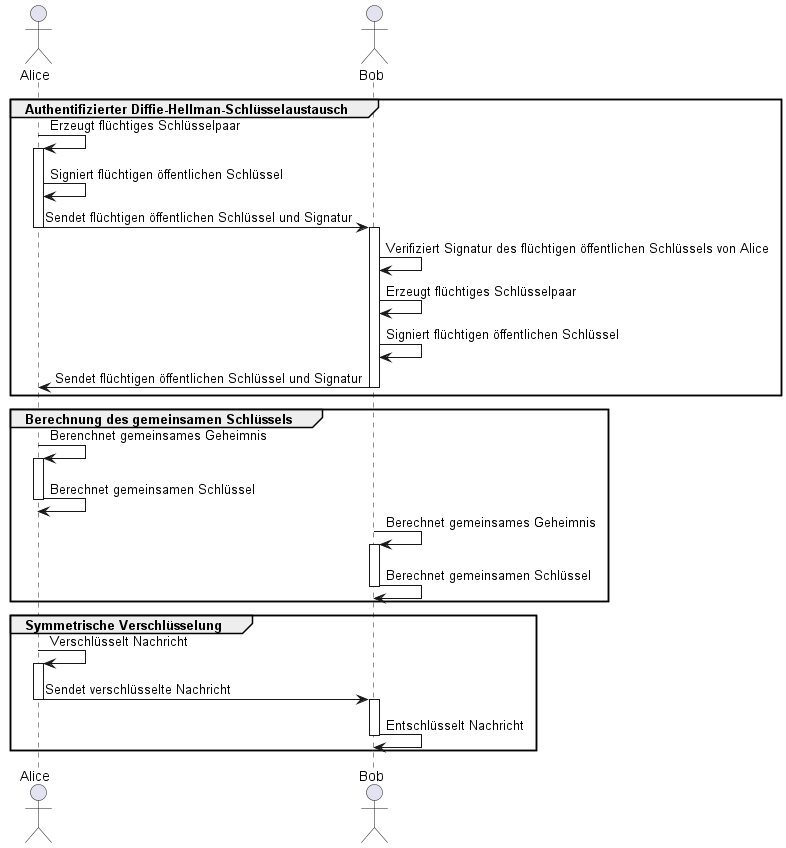
\includegraphics[width=1\linewidth]{images/sec.png}
    \caption{Modifizierte Ende-zu-Ende-Verschlüsselung}
    \label{fig:ende_zu_ende}
\end{figure}

\noindent Im Block \textit{Authentifizierter Diffie-Hellman Schlüsselaustausch} aus Abbildung \ref{fig:ende_zu_ende} erzeugt Alice ein neues X25519-Schlüsselpaar und signiert ihren öffentlichen Schlüssel unter Verwendung des privaten statischen Ed25519-Schlüssels. Dieser signierte öffentliche Schlüssel wird an Bob gesendet. Bob erzeugt ebenfalls ein X25519-Schlüsselpaar und signiert seinen öffentlichen Schlüssel mit seinem privaten statischen Ed25519-Schlüssel. Dieser signierte öffentliche Schlüssel wird an Alice gesendet. Alice und Bob können nun das gemeinsame Geheimnis berechnen (siehe \ref{fig:schluesselvereinbarung} \textit{\nameref{fig:schluesselvereinbarung}}) und damit den Double Ratchet Algorithmus initialisieren.


\subsection{Statische Schlüssel}
Die statischen Schlüssel werden verwendet, um die Teilnehmer zu authentifizieren (Berechnung und Verifikation der Signaturen). Diese Schlüssel werden einmalig bei der Registrierung (siehe \ref{subsec:identifikation_von_teilnehmern} \textit{\nameref{subsec:identifikation_von_teilnehmern}}) eines Teilnehmers erzeugt. Der private Schlüssel wird lokal auf dem Gerät des Teilnehmers gespeichert. Für den öffentlichen Schlüssel muss ein Weg gefunden werden, diesen allen anderen Teilnehmern öffentlich zugänglich und eindeutig zuordenbar zu machen. Hierfür wird die Blockchain verwendet. 

